%Dies ist die Hauptseite des Dokumentes. Es werden u. a. alle Kapitel,
%Einstellung im Header eingebunden.  Veränderungen müssen in folgenden Dateien
%vorgenommen werden:
      %- Layout.tex
      %- newComments.tex
      %- Titelseite
      %- Versionsübersicht
      %- einzelne Kapitel (evtl. erweitern)


% Definition von globalen Parametern, die derzeit auf der Titelseite und in der
% Kopfzeile verwendet werden. Der in <> gesetzte Text ist zu verändern.

\newcommand{\praktikumTitel}{WiRe}
\newcommand{\projektTitel}{Ctl-Web}


%Hier sind alle Einstellungen enthalten, die sich auf das Seiten- und
%Dokumentenlayout beziehen

\documentclass[
  11pt,                % Schriftgröße
  DIV12,
  german,              % für Umlaute, Silbentrennung etc.
  oneside,            % einseitiges Dokument
  titlepage,          % es wird eine Titelseite verwendet
  halfparskip,        % Abstand zwischen Absätzen (halbe Zeile)
  normalheadings,      % Größe der Überschriften verkleinern
  tablecaptionabove,  % Beschriftung von Tabellen unterhalb ausgeben
  final                % Status des Dokuments (final/draft)
]{scrreprt}            %


%------Ändern von Schriftschnitten - (Muss ganz am Anfang stehen !) ------------
\usepackage{fix-cm}

%------Umlaute -----------------------------------------------------------------
%   Umlaute/Sonderzeichen wie äüöß können direkt im Quelltext verwenden werden.
%    Erlaubt automatische Trennung von Worten mit Umlauten.
\usepackage[T1]{fontenc}
\usepackage[utf8]{inputenc}

%------Anpassung der Landessprache----------------------------------------------
\usepackage{ngerman}

%------Einfache Definition der Zeilenabstände und Seitenränder------------------
\usepackage{geometry}
\usepackage{setspace}

%------Schriftgrößenanpassung von einzelnen Textpassagen------------------------
\usepackage{relsize}

%------Trennlinien in Kopf- und Fusszeile
\usepackage[headsepline, footsepline, ilines]{scrpage2}

%------Grafiken-----------------------------------------------------------------
\usepackage{graphicx}

%------Packet zum Sperren, Unterstreichen und Hervorheben von Texten------------
\usepackage{soul}

%------ergänzende Schriftart----------------------------------------------------
\usepackage{helvet}

%------Lange Tabellen-----------------------------------------------------------
\usepackage{longtable}
\usepackage{array}
\usepackage{ragged2e}
\usepackage{lscape}

%------PDF-Optionen-------------------------------------------------------------
\usepackage[
  bookmarks,
  bookmarksopen=true,
  colorlinks=true,
  linkcolor=black,        % einfache interne Verknüpfungen
  anchorcolor=black,      % Ankertext
  citecolor=black,        % Verweise auf Literaturverzeichniseinträge im Text
  filecolor=black,        % Verknüpfungen, die lokale Dateien öffnen
  menucolor=black,        % Acrobat-Menüpunkte
  urlcolor=black,         % Farbe für URL-Links
  backref,                % Zurücktext nach jedem Bibliografie-Eintrag als
                          % Liste von Überschriftsnummern
  pagebackref,            % Zurücktext nach jedem Bibliografie-Eintrag als
                          % Liste von Seitenzahlen
  plainpages=false,       % zur korrekten Erstellung der Bookmarks
  pdfpagelabels,          % zur korrekten Erstellung der Bookmarks
  hypertexnames=false,    % zur korrekten Erstellung der Bookmarks
  linktocpage             % Seitenzahlen anstatt Text im Inhaltsverzeichnis
                          % verlinken
  ]{hyperref}



      % enthält eingebundene Packete

%------Seitenränder-------------------------------------------------------------
\geometry{verbose,                     % zeigt die eingestellten Parameter beim
                                       % Latexlauf an
      paper=a4paper,                   % Papierformat
      top=25mm,                        % Rand oben
      left=25mm,                       % Rand links
      right=25mm,                      % Rand rechts
      bottom=45mm,                     % Rand unten
      pdftex                           % schreibt das Papierformat in die
                                       % Ausgabe damit Ausgabeprogramm
                                       % Papiergröße erkennt
  }

%Seitenlayout
\onehalfspace        % 1,5-facher Abstand

%------Kopf- und Fußzeilen -----------------------------------------------------
\pagestyle{scrheadings}

%------Kopf- und Fußzeile auch auf Kapitelanfangsseiten ------------------------
\renewcommand*{\chapterpagestyle}{scrheadings}

%------Schriftform der Kopfzeile -----------------------------------------------
\renewcommand{\headfont}{\normalfont}

%------Kopfzeile----------------------------------------------------------------
\setlength{\headheight}{21mm}        % Höhe der Kopfzeile
\ihead{\large{\textsc{\praktikumTitel}}\\    % Text in der linken Box
       \small{\projektTitel}}
\chead{}                            % Text in der mittleren Box

%----Fusszeile
\cfoot{}                            % Text in mittlerer Box
\ofoot{\pagemark}                    % Seitenzahl in rechter Box

           % Diese Datei enthält alle
                                           % Layouteinstellungen

%------Beginn des Gesamtdokumentes----------------------------------------------

\begin{document}

%------Eingebundene Seiten, Verzeichnisse bzw. Kapitel--------------------------
% Dies ist die Titelseite des Pflichtenhefts.
% Die in "<...>" sind zu ersetzen
% Die Ausgabe darf 1 Seite nicht überschreiten, also ggf. Abstände anpassen
% Die Angabe in [...] gibt den Abstand nach der entsprechenden Zeile an.


%----Stil dieser Seite----------------------------------------------------------
\thispagestyle{plain}      % Kopfzeile bleibt leer

%----Beginn der Titelseite------------------------------------------------------
\begin{titlepage}

%----zentrierte Ausrichtung über die gesamte Seite----------------------------
\begin{center}

%----Titel des Praktikum (\praktikumTitel in newComments zu verändern)--------
{\relsize{4}{\textbf{\textsc{\praktikumTitel}}}}\\[3ex]%[5ex]

%----Titel des Teilprojektes (\projektTitel in newComments verändern)---------
{\relsize{3}{\textbf{\textsc{\projektTitel}}}}\\[3ex]%[5ex]

Teamprojekt\\
Wintersemester 2012/2013\\[4ex]%[6ex]

{\relsize{3}\so{\textbf{Pflichtenheft}}}\\[4ex]%[5ex]

%----eingebundenes Logo der TU--------------------------------------------------

\includegraphics[scale=0.8]{bilder/carolo.jpg}\\[4ex]%[5ex]

%----Daten des Auftraggebers
Auftraggeber\\
Technische Universität Braunschweig\\
Wissenschaftliches Rechnen\\
Prof. Hermann G. Matthies\\
Hans-Sommer-Straße 65\\
D-38092 Braunschweig\\[1ex]%[2ex]
Betreuer: Elmar Zander / Rainer Niekamp\\[4ex]%[5ex]

% ----Tabelle der Praktikumsteilnehmer------------------------------------------
Auftragnehmer:
\begin{tabular}{l<{\hspace{20mm}} l<{\hspace{30mm}}}\\
  Name                   &   E-Mail-Adresse\\      % Zeilenüberschift
  \hline                    % Linie unterhalb der Zeilenüberschrift
  %----Nachfolgend alle Namen und E-Mail-Adressen der Teilnehmer einfügen
  Eric Anders 		& eric.anders89@web.de\\
  Johann Hong 		& johann.hong@googlemail.com\\
  Jörn Hameyer 		& j.hameyer@tu-bs.de\\
  Marco Melzer 		& marco.melzer@tu-braunschweig.de\\
  Markus Dietrich 	& markus.dietrich@tu-bs.de\\
  Philipp Offensand & PhilippOffensand@gmx.de\\
  Stephan Sobol 	& stephan.sobol@web.de\\
  Theodor van Nahl 	& t.nahl@tu-bs.de
\end{tabular}\\[1ex]%[2ex]

Braunschweig, 30.11.2012

\end{center}
\end{titlepage}
                       % Titelseite
%Diese Datei dient der Versionskontrolle. Sie ist vollständig zu bearbeiten.

%----Überschrift------------------------------------------------------------
{\relsize{2}\textbf{Versionsübersicht}}\\[2ex]

%----Start der Tabelle------------------------------------------------------
\begin{longtable}{|m{1.78cm}|m{1.59cm}|m{2.86cm}|m{1.9cm}|m{5.25cm}|}

  \hline                                              % Linie oberhalb

  %----Spaltenüberschriften------------------------------------------------
  \textbf{Version}  &    \textbf{Datum}  &    \textbf{Autor}  &
  \textbf{Status}   &    \textbf{Kommentar}  \\  %Spaltenüberschrift
  \hline                                              % Gitterlinie

  %----die nachfolgeden beiden Zeilen so oft wiederholen und die ... mit den
  %    entsprechenden Daten zu füllen wie erforderlich
  ...    &    ...    &    ...    &    ...    &    ...\\       % Eintrag in Zeile
  \hline                                              % Gitterlinie unten

%----Ende der Tabelle------------------------------------------------------
\end{longtable}
Status: "`in Bearbeitung"' oder "`abgenommen"'\\
Kommentar: hier eintragen, was geändert bzw. ergänzt wurde



Hinweis zum Template:
Dieses Template enthält Beispiele und andere Hinweise, die alle kursiv
geschrieben sind. Alles Kursivgeschriebene ist selbstverständlich bei Abgabe zu
entfernen.

Angaben in <\ldots> sind mit dem entsprechendem Text zu füllen.

        % Versionsübersicht

\tableofcontents                           % Inhaltsverzeichnis wird automatisch
                                           % generiert
\listoffigures                             % ebenso das Abbildungsverzeichnis

%----Kapitel des Feinentwurfs, die mit Inhalt zu füllen sind--------------------
% Kapitel 1
% Die Unterkapitel können auch in separaten Dateien stehen,
% die dann mit dem \include-Befehl eingebunden werden.
%-------------------------------------------------------------------------------

\chapter{Zielbestimmung}

%Hier Einleitungstext einfügen, dabei die Formatierungen selber erstellen


Das Ziel unseres Projektes ist es, ein System zu erstellen, welches es unserer Benutzergruppe erlaubt, eigene Komponenten bereitzustellen bzw. Komponenten anderer im eigenen Projekt zu verwenden, sowie die Ausführung dieser Komponenten auf Computerclustern. Für die Anzeige der Komponenten wird ein Webinterface bereitgestellt, das Ausführen der Komponenten übernimmt ein zweites paralleles System.
Die Benutzergruppe umschließt vorerst die TU-Braunschweig, evtl. auch andere Universitäten sowie Institutionen. 
 

\section{Musskriterien}

%\begin{itemize}
%\item  Es muss eine Webfrontend geben um die Compontents einzusehen
%\item  Webfrontend muss initialen Quellcode Snippets bereit stellen.
%\item  Stabilität des Systems
%\item  Push für Manifest ins Frontend
%\item  Pull von Cluster der Manifestdateien
%\item  Upload von Manifest ins Frontend
%\end{itemize}

\begin{itemize}
\item Webinterface für die \glqq Discover \grqq , d.h. das Webinterface besitzt eine gut funktionierende Suche, welche dem Nutzer als Ergebnis die gewünschten Komponenten anzeigt
\item Die Detailseite der Komponenten enthält erste wichtige Informationen wie Name, Autor, Version etc. auf, weiterhin wird eine Quellcode
Snippet bereitgestellt
\item Rollen: 
\begin{description}
\item{Gast}kann nach Komponenten suchen, kann deren Details ansehen
\item{registrierter Nutzer} kann Komponenten bei sich einfügen, kann "Programme" mit diesen Fremdkomponenten starten
\item{Administrator} kann das Webinterface anpassen, d.h. Komponenten freischalten/löschen, Nutzer freischalten/löschen etc.
\end{description}
\item ein zweites System, welches die Verbindungen der Komponenten zu den Clustern bereitstellt
\end{itemize}

\paragraph{Benutzerdaten}

\begin{description}
	\item[Administrator] Alles
	\item[User]
		\begin{itemize}
			\item Kann Components ausführen
			\item Neue C hinzufügen
			\item Auslesen von C
			\item Login auf Webfrontend
		\end{itemize}
	\item[Gast] 
		\begin{itemize}
			\item Manifest lesen
			\item Kein Snippet-Code lesen
			\item Componten lesen
		\end{itemize}
\end{description}

\section{Wunschkriterien}

\begin{itemize}
\item  Absicherung des Zugriffes
\item  Anbindung von diesen Systemen untereinander (Social Programming)
\item  LDAP Anbindung
\item  Multilinguale Unterstützung
\end{itemize}

\section{Abgrenzungskriterien}

\begin{itemize}
\item  Social Programming wird nicht implemtiert, soll nur evtl. vorbereitet werden.
\item  Das System ist nicht für sehr große
\item  Es wird \emph{nur} English als Systemsprache zur Verfügung
\end{itemize}
            % Kapitel 1
%% Kapitel 2 mit den entsprechenden Unterkapiteln
% Die Unterkapitel können auch in separaten Dateien stehen,
% die dann mit dem \include-Befehl eingebunden werden.
%------------------------------------------------------------------------------------
\chapter{Produkteinsatz}
Dieser Abschnitt hat die Aufgabe, den Einsatzbereich, die Zielgruppen und die
Betriebsbedingungen des zu entwickelnden Systems klarzustellen.

\section{Anwendungsbereiche}
Hier wird der Bereich beschrieben, in dem das Produkt eingesetzt werden soll,
bzw. Bereiche, für die das Produkt nicht gedacht ist.

\section{Zielgruppen}
Hier wird angegeben, für welche Anwender (z. B. Sekretärin, andere Entwickler)
das Produkt im Wesentlichen gedacht bzw. nicht gedacht ist.

\section{Betriebsbedingungen}
Hier werden die unterschiedlichen Bedürfnisse und Anforderungen an das Produkt
aufgelistet. Dies können folgenden Punkte sein:
-  physikalische Umgebung des Systems (z. B. Büroumgebung, mobiler Einsatz)
-  tägliche Betriebszeit (z. B. Dauerbetrieb)
-  ständige Beobachtung des Systems durch einen Bediener oder unbeaufsichtigter
   Betrieb
            % Kapitel 2
% Kapitel 3
%-------------------------------------------------------------------------------
\chapter{Produktübersicht}

\begin{figure}[h]
\centering
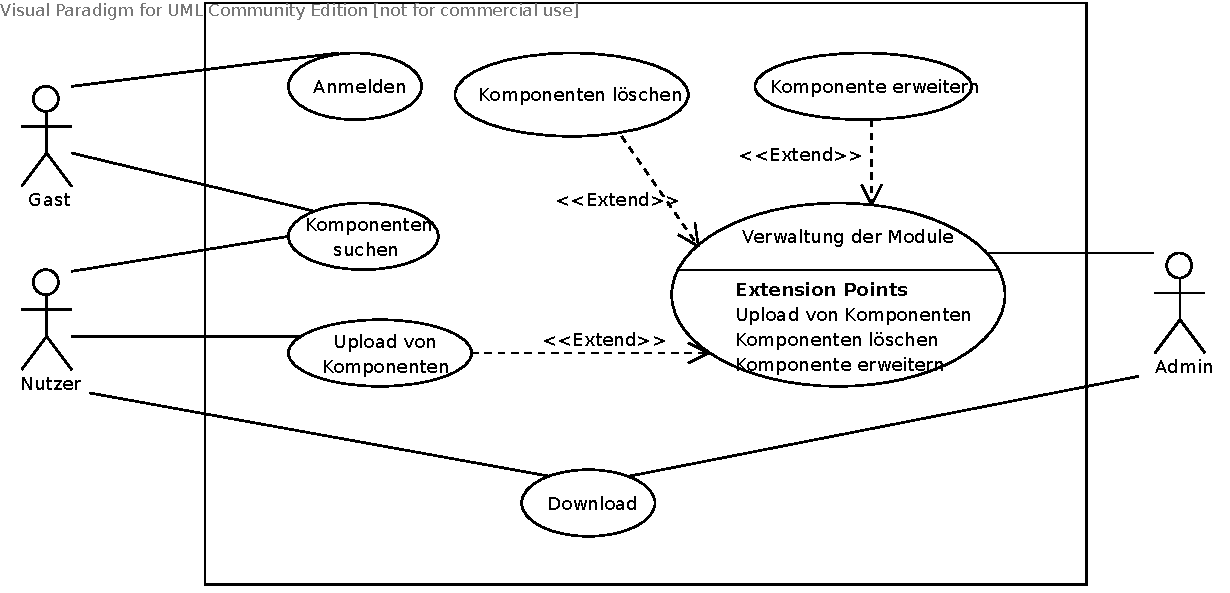
\includegraphics[width=0.8\linewidth]{bilder/Use-Case-Frontend.pdf}
\caption[Use-Case-Diagramm]{Use-Case-Diagramm}
\label{use-case}
\end{figure}
         % Kapitel 3
% Kapitel 4
%-------------------------------------------------------------------------------

\chapter{Produktfunktionen}

\section{Frontend Funktionen}
\subsection{F100 (Anmeldung)}
\label{F:Anmeldung}
\begin{description}
  \item[Ziel]Ein Benutzer meldet sich erfolgreich am System an.
  \item[Vorbedingung]Der Benutzer ist bereits auf dem System registriert und besitzt ein Passwort.
  \item[Akteure]Unangemeldeter Benutzer
   \item[Beschreibung]\hfill
    \begin{enumerate}
      \item Der Benutzer wählt den Link \emph{Login} auf der Webseite aus.
	  \item Der Benutzer kommt in ein Login-Fenster, in dem er Benutzer und
		Passwort eingeben kann und bestätigt dies mit einem Button.
	  \item Die Daten werden vom System überprüft und der Benutzer informiert
		ob der Login erfolgreich war.
	  \item Außerdem wird dem Benutzer irgendwo auf der Seite sein Login-Status
		angezeigt.
    \end{enumerate}
\end{description}

\subsection{F101 (Suche)}
\label{F:Suche}
\begin{description}
  \item[Ziel]Eine bestimmte Komponente wird gefunden
  \item[Vorbedingung]Der Benutzer ist angemeldet
  \item[Akteure] Angemeldeter Benutzer
   \item[Beschreibung]\hfill
    \begin{enumerate}
      \item Der Benutzer wählt den Link \emph{Suche} auf der Webseite aus.
	  \item Der Benutzer hat die Wahl zwischen zwei Suchverfahren.
	  \item Das Erste ist eine einzelne Eingabezeile in der mit logischen
		Begriffen gesucht werde kann.
	  \item Das Zweite besteht aus mehreren optionalen Suchfeldern, die
		relevante Eigenschaften der Komponenten repräsentieren. Hier kann der
		Benutzer gezielt nach Eigenschaften der Komponenten suchen.
	  \item Die Ergebnisse werden in einer übersichtlichen Tabelle mit den
		wichtigsten Eigenschaften angezeigt.
    \end{enumerate}
\end{description}

\subsection{F102 (Detailinformation der Komponenten)}
\label{F:Details}
\begin{description}
  \item[Ziel]Einem Benutzer werden Detailinformationen einer Komponente
	angezeigt.
  \item[Vorbedingung]Der angemeldete Benutzer besitzt z.B. durch Verwenden der Suche den
	Link zur Detailseite der Komponente.
  \item[Akteure]Angemeldeter Benutzer
   \item[Beschreibung]\hfill
    \begin{enumerate}
      \item Der Benutzer öffnet den Link zur Detailseite einer Komponente.
	  \item Dem Benutzer werden in tabellenartiger Form alle
		Detailinformationen angezeigt.
	  \item Der Benutzer erhält die Möglichkeit eine Verbindung zu der
		Komponente aufzubauen.
    \end{enumerate}
\end{description}

\subsection{F103 (Eintragung von Komponenten)}
\label{F:Eintragen}
\begin{description}
  \item[Ziel]Eine neue verfügbare Komponente wird eingetragen.
  \item[Vorbedingung]Der Benutzer ist als User angemeldet und hat alle
	relevanten Daten einer neuen Komponente, die bereitgestellt werden soll.
  \item[Akteure]Administrator
   \item[Beschreibung]\hfill
    \begin{enumerate}
      \item Der Benutzer wählt den Link \emph{Komponentenadministration} auf der Webseite aus.
	  \item Der Benutzer kommt in ein Fenster in dem er alle notwendigen und
		gewünschte zusätzliche Informationen einträgt.
	  \item Der Benutzer bestätigt die Informationen und das System trägt die
		neue Komponente in seine Datenbank ein.
	  \item Der Benutzer bekommt Informationen ob die Eintragung erfolgreich
		verlaufen ist.
    \end{enumerate}
\end{description}


\subsection{F104 (Bearbeiten von Komponenten)}
\label{F:Bearbeiten}
\begin{description}
  \item[Ziel]Eine Komponente wird bearbeitet oder gelöscht.
  \item[Vorbedingung]Der Benutzer ist als Administrator auf der Detailseite
	einer Komponente oder als User auf der Detailseite einer selbst eingetragenen
	Komponente.
  \item[Akteure]Administrator, User
   \item[Beschreibung]\hfill
    \begin{enumerate}
      \item Der Benutzer hat einen zusätzlichen Button zur Bearbeitung auf der
		Detailseite der Komponente.
	  \item Mit dem Button kommt der Benutzer auf eine Seite, auf der er alle
		relevanten Informationen ändern kann
	  \item Auf der Seite befindet sich ein Button zum Löschen der Komponente.
	  \item Der Benutzer bestätigt seine Änderungen mit einem bestimmten
		Button.
    \end{enumerate}
\end{description}

\begin{itemize}
	\item Login /Logout
	\item Suche nach Componten von Benutzern
	\item Manifest Push
	\item Manifest pull
	\item Manifest upload
	\item Snippet bereitstellung
	\item 
\end{itemize}<++>
         % Kapitel 4
% Kapitel 5
%------------------------------------------------------------------------------------------

\chapter{Produktdaten}

\begin{itemize}
	\item Manifest beschreiben
		\begin{itemize}
			\item Author
			\item Name
			\item Datum der Veröffentlichung
			\item Version
			\item Beschreibung
			\item Snippets
			\item Location
			\item Programmiersprache
		\end{itemize}<++>
	\item Inhalt der Datenbank beschreiben (Manifest + Benutzerdaten)
	\item gespeicherte Benutzerdaten
\end{itemize}
              % Kapitel 4
% Kapitel 6
%-------------------------------------------------------------------------------

\chapter{Nichtfunktionale Anforderungen}

\begin{itemize}
	\item Sicherheit steht nicht im Vordergrund
	\item Zuverlässigkeit steht an vorderster Stelle
	\item Benutzbarkeit sollte gegeben sein
	\item Stabilität muss gewährleistet sein
	\item Übertragbarkeit ist nicht relevant
\end{itemize}<++>
        % Kapitel 4
% Kapitel 7
%-------------------------------------------------------------------------------


\chapter{Benutzeroberfläche}

Die Benutzeroberfläche wird unterteilt in mindestens drei Webseiten:
Ausgehend von einer Suchseite, werden die Ergebnisse tabellarisch unter der
Suchmaske angezeigt, die auf Detailseiten weiterführen. 
Der Benutzer hat je nach Rechtestatus eine Gast-/Benutzer- oder eine Administrationsumgebung (zum Beispiel zum normalen Einsehen, Verändern, Löschen von Komponenten). 

\section{/B10/ Seitenlayout}

 \begin{itemize}
   \item Komponentendatenbank
   \begin{itemize}
    \item Suche
      \begin{description}
       \item[Einfache Suche] Die einfache Suche soll relativ unkompliziert funktionieren:
        Sie besteht lediglich aus einer Eingabefläche, worin der Benutzer
       den Namen der Komponente, Autoren oder Sonstiges eingeben kann. 
       \item[Erweiterte Suche] Die erweiterte Suche stellt mehrere Optionen zur Verfügung, um die Suche zu präzisieren. 
       \end{description}
    \end{itemize}
    \item Verzeichnis
      \begin{description}
        \item[] Hier findet der Benutzer eine Liste von den verfügbaren Interfaces und ihren zugehörigen Komponenten.
        Durch Auswählen einer bestimmten Komponente, wird der Benutzer zu ihrer Detailseite weitergeleitet.
        Dort findet er neben der Beschreibung eine Übersicht zu den verantwortlichen Programmieren, der Versionsnummer, das Erstelldatum und auf welchem Server sich die betrachtete Komponente befindet. 
        Dem Benutzer wird zudem ein Link angeboten, um die gewünschte Komponente bei sich zu integrieren. 
      \end{description} 

    \item Anmeldung/Registrierung
      \begin{description}
        \item[Login] Der Benutzer kann sich mit seinem Benutzernamen/Passwort anmelden. Sollte er sein Passwort vergessen haben, gibt die Seite ihm per Eingabe seiner Mailadresse die Gelegenheit, sich ein Neues setzen zu lassen.
        \item[Registrieren]Der Benutzer kann sich mit einem beliebigen Benutzernamen und Passwort registrieren, die eine Emailadresse erfordert. 
      \end{description}   
    
    \item Administration
      \begin{description}
        \item[] test
      \end{description}
 \end{itemize}
 
\begin{figure}
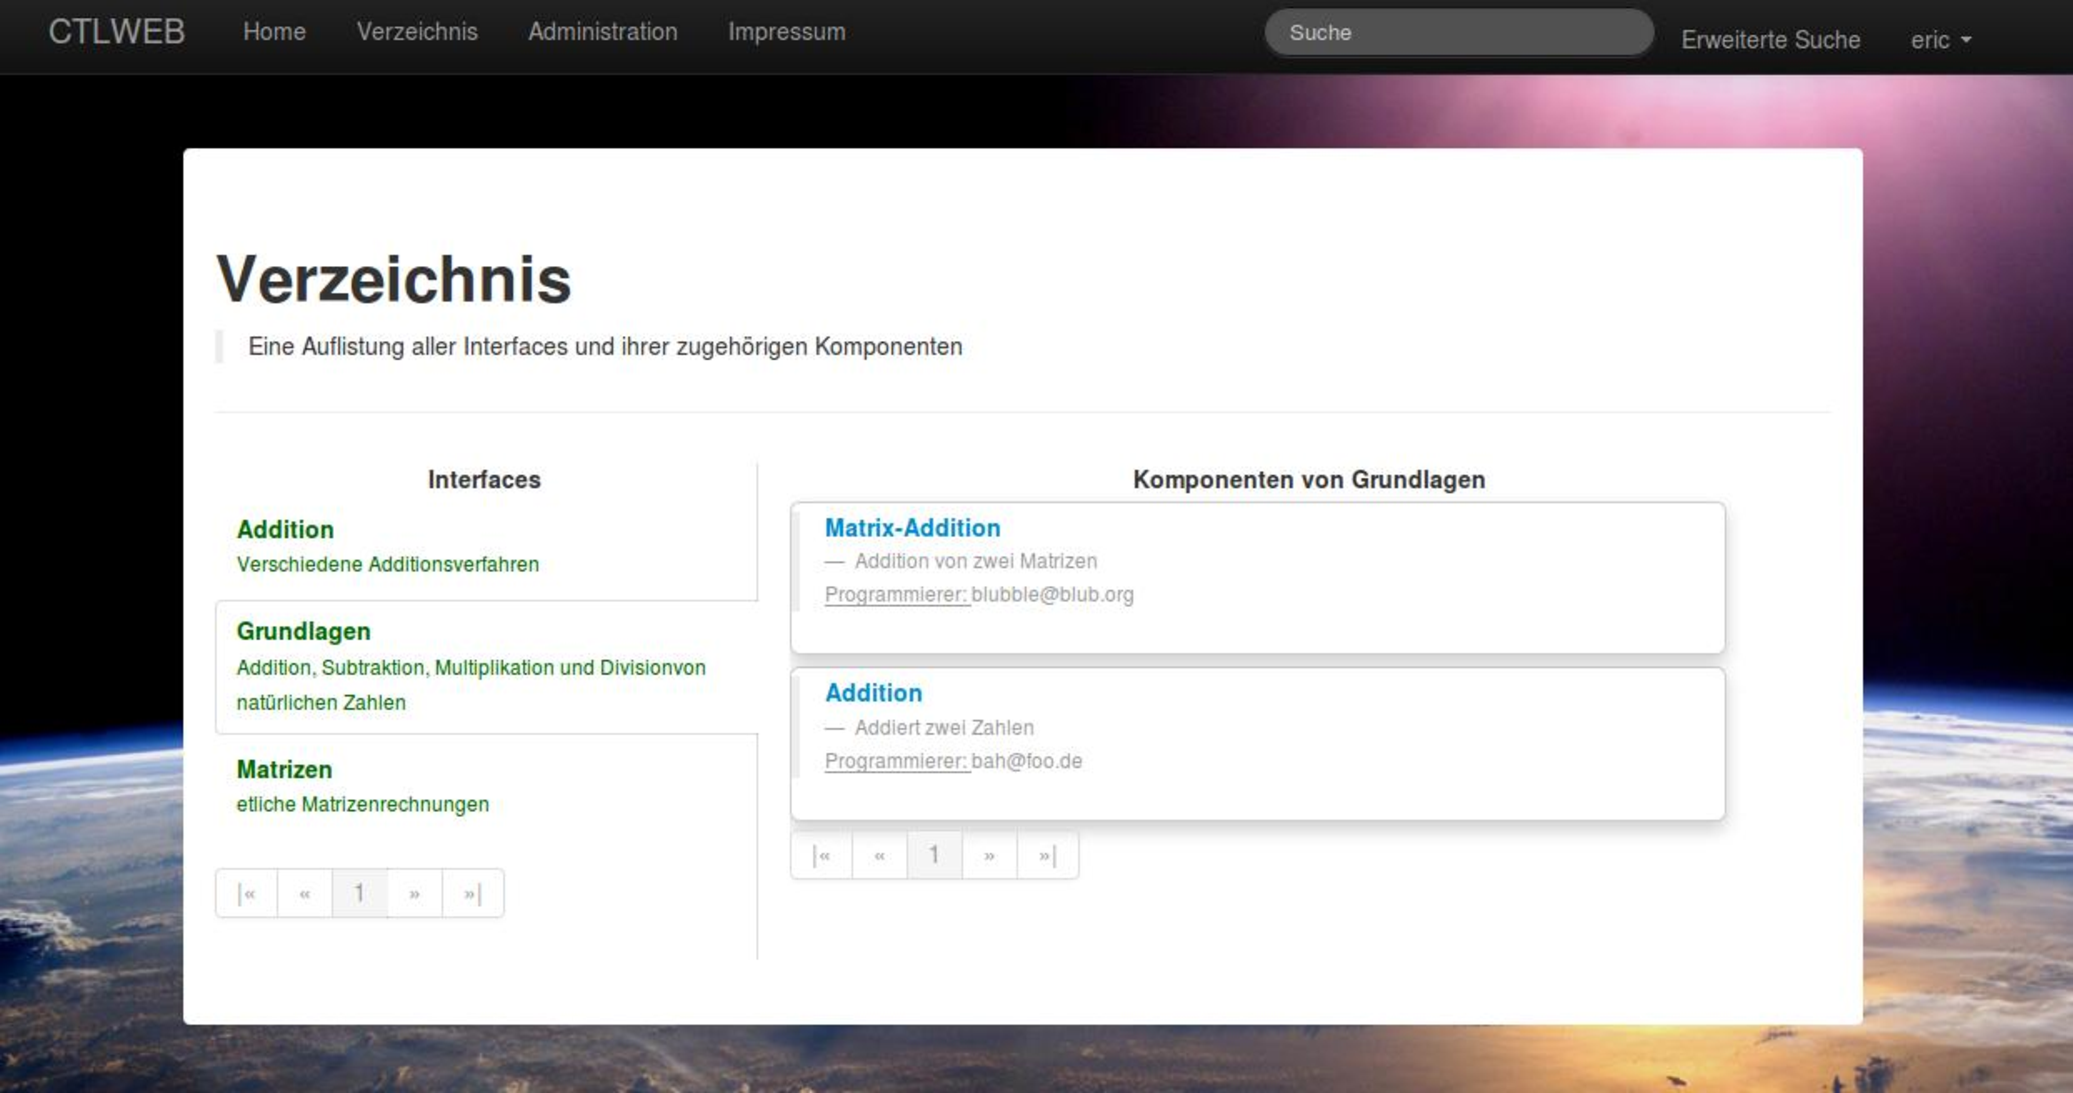
\includegraphics[width=0.8\linewidth]{bilder/ctlweb.pdf}
\caption{Beispiel für ein Seitenlayout}
\label{fig:gui}
\end{figure}

Suchergebnisse werden in einem großen Bereich rechts bzw.\ unter der Navigation angezeigt. 
Die Komponenten werden übersichtlich in tabellenartiger Form bereitgestellt. Bei einem Klick auf ein bestimmtes Suchergebnisses erscheinen genauere Informationen über die Komponente. 
Oben rechts wird zudem der eingeloggte User angezeigt.
Bei einem Klick auf den eingeloggten User ist eine Account-Verwaltungsseite geplant.
       % Kapitel 4
% Kapitel 10
% Die Unterkapitel können auch in separaten Dateien stehen,
% die dann mit dem \include-Befehl eingebunden werden.
%-------------------------------------------------------------------------------

\chapter{Technische Produktumgebung}

In diesem Kapitel wird die technische Umgebung des Produktes beschrieben. Bei
Client / Server - Anwendungen ist die Umgebung jeweils für Client und Server
getrennt anzugeben.

\section{Software}
Hier wird angegeben, welche Softwaresysteme (z. B. Betriebssystem, Datenbank,
Fenstersystem, usw.) zur Verfügung stehen.\\

Beispiel:\\
Server-Betriebssystem: Linux.\\
Client-Betriebssystem: Windows XP oder Browser (für Fernwartung).\\


\section{Hardware}
Hier werden die Hardware Komponenten (z. B. CPU, Peripherie) in minimaler und
maximaler Konfiguration aufgeführt, die für den Produkteinsatz vorgesehen
sind.\\
Beispiel:\\
Server: PC\\
Client: PC und browserfähiges Gerät mit Grafikbildschirm (für Fernwartung).


\section{Orgware}
Hier wird aufgeführt, unter welchen organisatorischen Randbedingungen bzw.
Voraussetzungen das Produkt eingesetzt werden soll.
Beispiel:\\
Netzwerkverbindung des Servers zum Computersystem der Testmaschinen, von dem
die Abmeldung der Reifen nach durchgeführtem Testlauf kommt.



\section{Produktschnittstellen}
Wird das Produkt in eine bestehende oder geplante Produktfamilie eingeordnet,
so werden hier die entsprechenden Schnittstellen definiert.
Beispiel:\\
Die Kommunikation mit der unterlagerten SPS erfolgt über getrennt definiertes
(eigenes Pflichtenheft) TCP/IP - Protokoll. Analoges gilt für die Kommunikation
mit dem Testmaschinen-Rechner.
           % Kapitel 4
% Hier wird das Deployment beschrieben.
% --------------------------------------------------------------------

\chapter{Deployment}
\section{Frontend}
Folgende Pakete werden für die funktionsfähigkeit der Webseite benötigt:
  \begin{itemize}
	\item paramiko
	\item django 1.3
	\item django-registration
  \end{itemize}


Zuerst muss das Projekt geforkt werden. Dazu im gewünschten Ordner den Befehl '
git clone https://github.com/ctldev/ctlweb.git' ausführen. Im Ordner des
Projektes befindet sich im Subordner 'src/frontend' die manage.py von Django.
Hier sollte der Befehl 'python manage.py create\_impressum' ausgeführt werden,
um ein personalisiertes Impressum zu generieren. Alternativ muss ein eigenes 
in dem Ordner 'src/frontend/template' mit dem Namen
'personal\_impressum.html' generiert werden. Nun kann die Webseite gestartet
werden.
Auf der Webseite sollten nun in der Admin-Section die Cluster hinzugefügt werden,
auf denen sich die darzustellenden Komponenten befinden. Die Komponenten des
Clusters lassen sich über den Befehl 'python manage.py request\_modules'
abfragen. Regelmäßige Abfragen sind so auch zum Beispiel über einen Cron-Job
oder Ähnliches zu realisieren.
\section{Backend}
Folgendes Paket wird für die Funktionsfähigkeit des Programms benötigt:
\begin{itemize}
  \item requests (python3)
\end{itemize}

% Kapitel 9
%-------------------------------------------------------------------------------

\chapter{Glossar}
Hier werden Fachbegriffe erklärt.

%------Ende des Dokumentes------------------------------------------------------
\end{document}
